\documentclass{article}

% PACKAGES
\usepackage[margin=1in]{geometry} % For setting page margins
\usepackage{graphicx}             % For including images
\usepackage{hyperref}             % For hyperlinks (optional, but good practice)
\usepackage{amsmath, amssymb}
\usepackage{amsfonts}
\usepackage{graphicx}
\usepackage{booktabs} % For professional-looking tables
\usepackage{xcolor}   % For colored boxes
\usepackage{listings}

\begin{document}

\section{Overview}

This section summarizes the data, notation, and end-to-end pipeline used to simulate and learn patient-specific lung deformation from 4D--CT. All symbols introduced here are reused consistently in later sections.
\newline
we denote 
\[
  \mathbf{u}_{\mathrm{true}} \colon \Omega \subset \mathbb{R}^3 \to \mathbb{R}^3
\]
the displacement field computed by non-rigid image registration between a \emph{reference} phase (typically end-exhalation, EE) and a \emph{target} phase (e.g., end-inspiration, EI). At each location $\mathbf{x}\in\Omega$, the vectors $\mathbf{u}_{\mathrm{true}}(\mathbf{x})$ specifies how the reference image must move to align with the target.

\subsection{Data specification}
\label{data-spec}

The primary entities manipulated by our framework are listed in Table~\ref{tab:data}. Note that the \emph{volumetric mesh is generated only once during preprocessing and reused for all respiratory phases}, whereas the displacement field is recomputed for each reference–target pair.

\begin{table}[h!]
\centering
\caption{Data entities used by the pipeline}
\label{tab:data}
\begin{tabular}{@{}lp{10cm}@{}}
\toprule
\textbf{Symbol / File} & \textbf{Description} \\
\midrule
$I_i\colon \Omega \to \mathbb{R}$ & 3D CT volume at respiratory phase $i$ (0\%, 10\%, \dots, 90\%), where 0\% corresponds to EE and 50\% to EI. \\[0.6em]
Segmentation mask & multi-class volume (same resolution as $I_i$) identifying lung parenchyma, airways, etc. Used to \emph{define the computational domain} and extract the surface $\partial\Omega$. \\[0.6em]
Volumetric mesh $\mathcal{T}=(\mathbf{V},\mathbf{E},\mathbf{T})$ & Generated once from the segmentation mask; provides vertices, edges, and tetrahedra for the mass–spring system. \\[0.6em]
Ground-truth displacement $\mathbf{u}_{\mathrm{true}}$ & Dense vector field obtained by solving the registration problem in Eq.~\eqref{eq:registration}. Interpolated (cubic or a first order (linear) B-spline in implementation)on $\partial\Omega$ to prescribe Dirichlet conditions. \\[0.6em]
Material labels $c(v)$ or intensities $I(v)$ & Node-/element-wise features consumed by the neural network that predicts stiffness. \\
\bottomrule
\end{tabular}
\end{table}


\textbf{Segmentation vs.\ boundary conditions.}  
A segmentation mask encodes \emph{shape only}. First it yields the surface geometry $\partial\Omega$ (via marching cubes). Then the independently computed registration field $\mathbf{u}_{\mathrm{true}}$ is sampled at each surface vertex to obtain the vector-valued data. Hence:
\begin{enumerate}
  \item \emph{Segmentation} $\longrightarrow$ domain $\Omega$ and boundary mesh;
  \item \emph{Registration} $\longrightarrow$ displacement vectors on $\Omega$;
  \item Sampling $\mathbf{u}_{\mathrm{true}}$ on $\partial\Omega$ $\longrightarrow$ prescribed displacements $\mathbf{u}_i$.
\end{enumerate}
The simulator never consumes the mask directly as a boundary condition.
\newline
\textbf{Image registration}


For a given pair $(I_{\mathrm{ref}}, I_{\mathrm{tar}})$, we estimate $\mathbf{u}_{\mathrm{true}}$ by solving
\begin{equation}
\label{eq:registration}
\min_{\mathbf{u}}
  \int_{\Omega} \bigl|I_{\mathrm{tar}}(\mathbf{x}) - I_{\mathrm{ref}}(\mathbf{x} + \mathbf{u}(\mathbf{x}))\bigr|^2 \,\mathrm{d}\mathbf{x}
  + \lambda \int_{\Omega} \lVert\nabla \mathbf{u}(\mathbf{x})\rVert^2 \,\mathrm{d}\mathbf{x},
\end{equation}
with $\lambda\in[10^{-2},10^{-1}]$.The result has been processed and stored as data. 



\subsection{Processing pipeline}
\label{ssec:pipeline}

\begin{table}[h]
\centering
\caption{End-to-end processing steps}
\label{tab:pipeline}
\begin{tabular}{@{}p{1.5cm}p{4.5cm}p{7.5cm}@{}}
\toprule
\textbf{Step} & \textbf{Input \(\to\) Output} & \textbf{Key operation} \\
\midrule
1 & \((I_{\mathrm{ref}},I_{\mathrm{tar}})\to\mathbf{u}_{\mathrm{true}}\) &
 Solve~\eqref{eq:registration}; saved as files. \\[0.4em]
2 & Mask \(\to \mathcal{T}\) &
 Generate tetrahedral mesh (cached). \\[0.4em]
3 & \(k \to \mathbf{u}_{\mathrm{sim}} = g(k)\) &
 Forward spring–mass solve (Sect.~\ref{sec:sms}):  
 enforce \(\nabla_{\mathbf{q}}U(k,\mathbf{q}) = \mathbf{0}\),  
 then compute \(\mathbf{u}_{\mathrm{sim}} = \mathbf{q} - \mathbf{X}.\) \\[0.4em]
4 & \(\mathbf{u}_{\mathrm{true}}\to k^*\) &  
 \(\displaystyle
   k^* = \arg\min_k \Bigl\lVert \mathbf{u}_{\mathrm{true}}
   - \mathbf{u}_{\mathrm{sim}}(k)\Bigr\rVert^2
 \)\\[0.8em]
5 & \((I_i, k^*)\to \theta^*\) &
 \emph{Learning}: train ANN \(k_\theta = f_\theta(I)\) via
 \(\displaystyle
   \theta^* = \arg\min_\theta 
   \mathbb{E}_{\mathrm{cases}}
   \Bigl\lVert \mathbf{u}_{\mathrm{true}}
   - \mathbf{u}_{\mathrm{sim}}\bigl(f_\theta(I)\bigr)\Bigr\rVert^2.
 \) \\
\bottomrule
\end{tabular}
\end{table}


\paragraph{Level 1 (Forward).}
Given a stiffness field \(k(\mathbf{x})\), solve for the simulated displacement:
\[
  g(k):\quad
  \frac{\partial U(k,\mathbf{q})}{\partial \mathbf{q}} = \mathbf{0},
  \qquad
  \mathbf{u}_{\mathrm{sim}} = \mathbf{q} - \mathbf{X}.
\]
Here:
\begin{itemize}
  \item Given the deformed nodal coordinates \(\mathbf{q}\in\mathbb{R}^{3N}\), 
  and the reference (initial) nodal coordinates \(\mathbf{X}\in\mathbb{R}^{3N}\).
  \item \(U(k,\mathbf{q})\) is the total potential energy (sum of all spring energies), 
  where $k$ is the stiffness field. 
  
  \item \(\nabla_{\mathbf{q}}U = \partial U/\partial \mathbf{q}\) is the gradient w.r.t.\, the nodal  \(\mathbf{q}\) forces; equilibrium makes the summarization zero.
  \item Get the simulated displacement field with \(\mathbf{u}_{\mathrm{sim}} = \mathbf{q}-\mathbf{X}\) .
\end{itemize}

\textbf{Level 2}
So we need to find \(k\) s.t.:
\[
  k^* = \arg\min_k
    \bigl\lVert \mathbf{u}_{\mathrm{true}}
    - \mathbf{u}_{\mathrm{sim}}(k)\bigr\rVert^2
,
\]




\textbf{Level 3 (Learning).}
Learn a mapping from image to stiffness:
\[
  \theta^* = \arg\min_\theta
    \mathbb{E}_{\mathrm{cases}}
    \bigl\lVert \mathbf{u}_{\mathrm{true}}
    - \mathbf{u}_{\mathrm{sim}}\bigl(f_\theta(I)\bigr)\bigr\rVert^2,
\]
with \(k_\theta = f_\theta(I)\) the ANN prediction and gradients flowing through the differentiable solver \(g(\cdot)\).






\section{Spring Mass System Approach}

For the forward simulation (Level 1), we model the deformable tissue, such as the lung, as a Mass-Spring System (MSM). 
The system consists of a grid of particles (mass points) interconnected by a network of springs. 
This model approximates the continuous mechanics of the tissue. Usually we need three steps to update the system:
\begin{enumerate}
  \item build the topology of the mass spring system
  \item Compute the forces based on the previous topology and act on each particle
  \item Integrate these forces over time to update the particle positions and velocities. Repeat the process for each time step until the simulation reaches a desired state or time.
\end{enumerate}
This section includes how we assemble the 
whole system from the aspect of total potential energy coming from the defined-topology springs.
The logic of the section is as follows: Firstly, we talk about the usual concepts of a mass-spring system, including
how to compute the spring forces and how to update the system forward. 
Then we introduce the topology of the volumetric mesh, which is a tetrahedral mesh, 
and how to compute the forces and use them to update the whole system.



\subsection{Introduction to Mass–Spring Systems}

In this section we outline the classical pipeline for a mass–spring system (SMS) simulation in three logical steps:

\begin{enumerate}
  \item \textbf{Build the topology of the mass–spring system.}
  \item \textbf{From the energy perspective, compute forces on each particle.}
  \item \textbf{Integrate these forces over time to update positions and velocities.}
\end{enumerate}

\paragraph{Particle definitions}  
We consider a 3D grid of \(N\) particles.  Each particle \(i\) has
\begin{itemize}
  \item \textbf{Mass} \(m_i\).  For simplicity we set \(m_i = m\) for all \(i\).
  \item \textbf{Position} \(\mathbf{x}_i(t)\in\mathbb{R}^3\).  Collectively \(\mathbf{x}=(\mathbf{x}_1,\dots,\mathbf{x}_N)\in\mathbb{R}^{3N}\).
  \item \textbf{Velocity} \(\mathbf{v}_i(t)=\dot{\mathbf{x}}_i(t)\).
\end{itemize}

\paragraph{1. Topology}  
We connect particles by three types of springs based on their grid indices \((i,j,k)\):
\begin{itemize}
  \item \textbf{Structural springs:} between \((i,j,k)\) and \((i+1,j,k)\), \((i,j+1,k)\), \((i,j,k+1)\).
  \item \textbf{Shear springs:} between diagonal neighbors, e.g.\ \((i,j,k)\) and \((i+1,j+1,k)\), etc.
  \item \textbf{Bend (flexion) springs:} between particles two steps away, e.g.\ \((i,j,k)\) and \((i+2,j,k)\).
\end{itemize}

\begin{figure}[!ht]
  \centering
  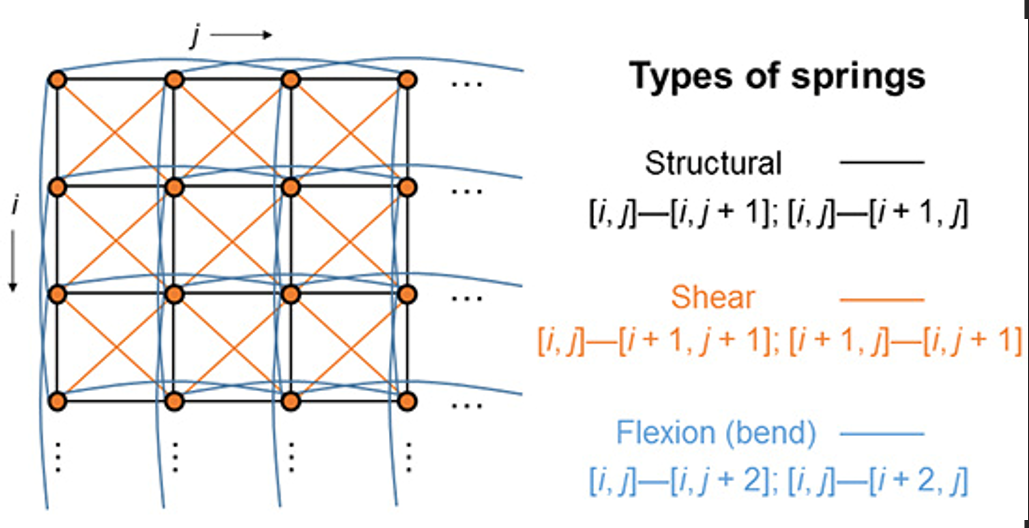
\includegraphics[width=0.8\textwidth]{images/fig2.0.png}
  \caption{Example mass–spring topology for a thin cloth patch.}
  \label{fig:simple_mass_spring}
\end{figure}

\paragraph{2. Forces from Energy}  
Each spring contributes a potential energy
\[
  U_{\rm spring}(\mathbf{p},\mathbf{q})
  = \tfrac12\,k\bigl(\|\mathbf{p}-\mathbf{q}\| - L_0\bigr)^2,
\]
where \(\mathbf{p},\mathbf{q}\) are its endpoint positions, \(k\) its stiffness, and \(L_0\) the rest length.  
The total elastic energy is
\[
  U(\mathbf{x})
  = \sum_{\text{springs } (i,j)} \tfrac12\,k_{ij}\bigl(\|\mathbf{x}_i-\mathbf{x}_j\| - L_{0,ij}\bigr)^2.
\]
The internal spring force on particle \(i\) is the negative energy gradient:
\[
  \mathbf{F}_i^{\rm int}
  = -\,\frac{\partial U}{\partial \mathbf{x}_i}
  = \sum_{j\in\mathcal{N}(i)}
    k_{ij}\bigl(L_{0,ij}-\|\mathbf{x}_i-\mathbf{x}_j\|\bigr)\,
    \frac{\mathbf{x}_i-\mathbf{x}_j}{\|\mathbf{x}_i-\mathbf{x}_j\|}.
\]

It's the same as the spring force in Hooke's law, where the force is proportional to the displacement from the rest length, and acts along the line connecting the two particles.:
\paragraph{Spring Forces}
Consider the internal force as the sum of forces from all springs connected to particle $i$. For a single spring connecting two particles at positions $\mathbf{p}$ and $\mathbf{q}$, with stiffness $k$ and rest length $L_0$, the restoring force exerted on particle $\mathbf{p}$ is given by Hooke's Law:
\begin{equation} \label{eq:spring_force}
    \mathbf{F}_{\text{spring}} = k (L_0 - \lVert \mathbf{p} - \mathbf{q} \rVert) \frac{\mathbf{p} - \mathbf{q}}{\lVert \mathbf{p} - \mathbf{q} \rVert}
\end{equation}
\newline
External forces (e.g.\ gravity \(\mathbf{F}_i^{\rm ext}=m\,\mathbf{g}\), contact, boundary constraints) are added to form the net force
\[
  \mathbf{F}_i(\mathbf{x},\mathbf{v})
  = \mathbf{F}_i^{\rm int} + \mathbf{F}_i^{\rm ext}.
\]

\paragraph{3. System Update}  
Particle motion obeys Newton’s second law:
\begin{equation}
  m_i\,\ddot{\mathbf{x}}_i(t)
  = \mathbf{F}_i\bigl(\mathbf{x}(t),\mathbf{v}(t)\bigr).
\end{equation}
A simple explicit Euler scheme with time step \(\Delta t\) reads
\[
  \mathbf{v}_i(t+\Delta t)
    = \mathbf{v}_i(t)
    + \frac{\Delta t}{m_i}\,\mathbf{F}_i\bigl(\mathbf{x}(t),\mathbf{v}(t)\bigr),
  \quad
  \mathbf{x}_i(t+\Delta t)
    = \mathbf{x}_i(t) + \Delta t\;\mathbf{v}_i(t).
\]
This loop (build topology–compute forces–integrate) is repeated each time step until the simulation reaches its target time or state.
Here the right‐hand sides are evaluated at time \(t\). Explicit Euler is easy to implement but conditionally stable (requires small \(\Delta t\)).


\subsection{Topology for volumetric mesh}
\textbf{Intersection Points \& Coefficient Matrix}

In each tetrahedral element $\mathcal V_k$, we locate six intersection points $q_{j}$\cite{bourguignon2000anisotropy, lakhal2013modified}
 by ray-casting from the \textbf{barycenter} $x_b$ along the three anisotropy axes to the faces. At the same time we build a $4\times6$ coefficient matrix $C^k$ whose entries let us reconstruct any intersection $q_j$ from the four vertex positions.

\begin{enumerate}
    \item \textbf{Barycenter}
    
    where $x_i$ are the four vertex coordinates.
    \begin{equation}
        x_b \;=\;\frac{1}{4}\sum_{i=1}^4 x_i
        \tag{2.22}
        \label{eq:barycenter}
    \end{equation}

    \item \textbf{Point-in-triangle test \& barycentric coords}
    
    A traced point $q_j$ on face $\Delta_{i_1i_2i_3}$ is inside if and only if
    \begin{equation}
        S_{\Delta_{i_1i_2i_3}} \;=\; S_{\Delta_{q_j\,i_2\,i_3}} + S_{\Delta_{i_1\,q_j\,i_3}} + S_{\Delta_{i_1\,i_2\,q_j}}.
        \tag{2.23}
        \label{eq:point_in_triangle}
    \end{equation}
    Then its local (area) coordinates on that triangle are
    \begin{equation}
        \xi=\frac{S_{\Delta_{q_j\,i_2\,i_3}}}{S_{\Delta_{i_1i_2i_3}}},\quad
        \eta=\frac{S_{\Delta_{q_j\,i_1\,i_3}}}{S_{\Delta_{i_1i_2i_3}}}, \quad
        1-\xi-\eta=\frac{S_{\Delta_{i_1\,i_2\,q_j}}}{S_{\Delta_{i_1i_2i_3}}}.
        \tag{2.24}
        \label{eq:barycentric_coords}
    \end{equation}
    
    \item \textbf{Building the coefficient matrix $C^k$}
    \begin{figure}[!ht]
    \centering
    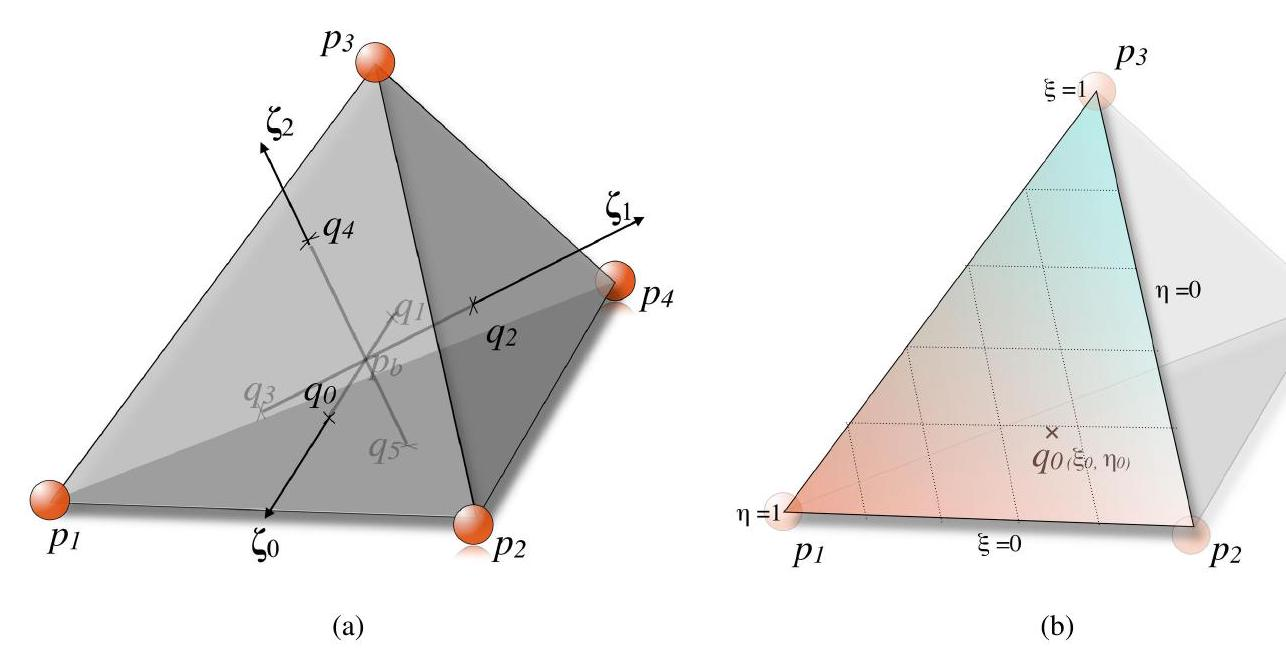
\includegraphics[width=0.8\textwidth]{images/fig2.6.jpg}
    \caption{Intersection points in a tetrahedral volume element: The tetrahedron with three axes of anisotropy set at the barycenter and the six intersection points that they define (a), a triangular face of the element containing an intersection point and the coefficients $\xi_{0}$ and $\eta_{0}$ related to the intersection point. Note that $\xi$ increases with the cyan color gradient starting from $\xi=0$ at the line segment ($p_{1}, p_{2}$) and is equal to $\xi=1$ at $p_{3}$, while $\eta$ increases along the orange color gradient starting from $\eta=0$ at ($p_{2}, p_{3}$) until it reaches $\eta=1$ at $p_{1}$ (b).}
    \label{fig:intersections}
\end{figure}

    For each intersection $q_j$ we evaluate the four linear shape-functions $N_i$ of the tetrahedron’s nodes $i=1\ldots4$. On the face containing $q_j$, those coincide with the barycentric coordinates:
    $$
    \begin{cases}
        N_{i_1}(q_j)=1-\xi-\eta,\\
        N_{i_2}(q_j)=\xi,\\
        N_{i_3}(q_j)=\eta,\\
        N_{i_4}(q_j)=0,
    \end{cases}
    $$
    where $\{i_1,i_2,i_3\}$ are the face nodes and $i_4$ is the opposite vertex. We then set
    $$
    C^k_{ij}\;=\;N_i\bigl(q_j\bigr),
    $$
    assembling a $4\times6$ matrix whose $j$-th column holds the four shape-function values at $q_j$.

    \item \textbf{Updating intersections}
    
    At runtime, once the current vertex positions $x^t_i$ are known, each intersection moves as
    \begin{equation}
        x^t_j \;=\;\sum_{i=1}^4 C^k_{ij}\;x^t_i
        \tag{2.25}
        \label{eq:update_intersections}
    \end{equation}
    reproducing the straight-sided mapping of a linear tetrahedron.
    
    In the implementation the six $q_j$ and the corresponding $C_k$
  are updated each step to remain exact under large deformation.
\end{enumerate}

\subsection{Internal Forces}

Internal (“deformation”) forces in each tetrahedron are computed by \textbf{three axial springs} along the anisotropy axes, plus \textbf{three torsion springs} coupling each pair of axes. See Fig. \ref{fig:springs}. The angle $\alpha_{\mathrm{lm}}^{t}$ between the axes $\zeta_{\mathrm{l}}$ and $\zeta_{\mathrm{m}}$ can be given by... % This sentence from the prompt seems incomplete.

\begin{figure}[ht!]
    \centering
    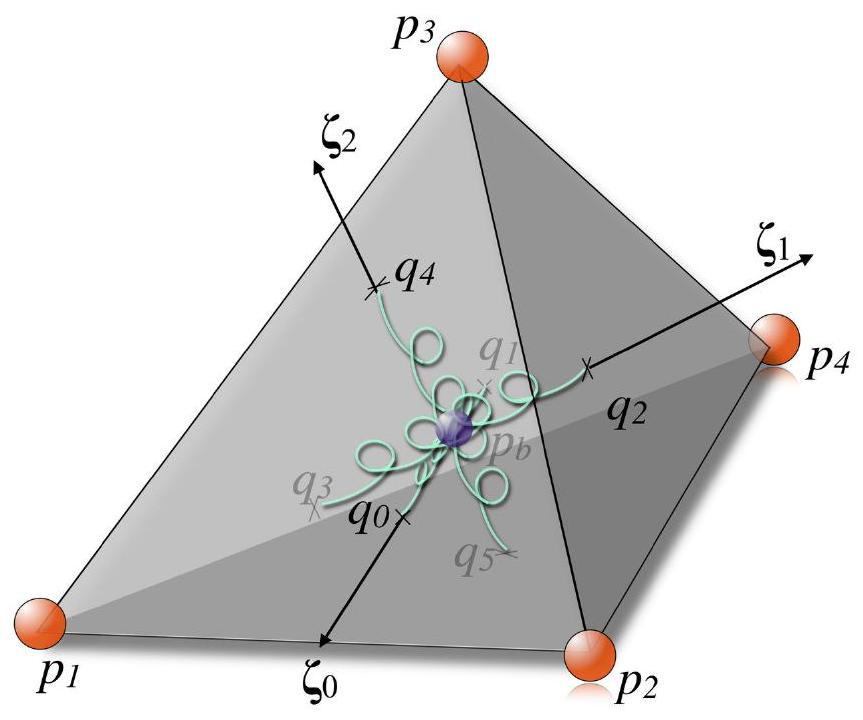
\includegraphics[width=0.5\textwidth]{images/fig2.12.jpg}
    \caption{A tetrahedron with three axial springs (in cyan) along the axes of anisotropy and three torsion springs in the barycenter of the tetrahedron (in violet).}
    \label{fig:springs}
\end{figure}

\subsubsection{Axial Springs}
\begin{itemize}
    \item \textbf{Axis vectors}: Along axis $\ell\in\{1,2,3\}$, let the two intersection points be $q_{\ell,1}$ and $q_{\ell,2}$. Their current axis vector is
    $$
    \zeta_\ell^t = x^t_{q_{\ell,1}} - x^t_{q_{\ell,2}}.
    $$
    
    \item \textbf{Initial length} (at $t=0$):
    \begin{equation}
    l^0_\ell = \|\zeta_\ell^0\| = \bigl\|\,x^0_{q_{\ell,1}}-x^0_{q_{\ell,2}}\,\bigr\|.
    \tag{2.30}
    \label{eq:initial_length}
    \end{equation}
    
    \item \textbf{Unit direction}:
    \begin{equation}
    \hat\zeta_\ell^t = \frac{\zeta_\ell^t}{\|\zeta_\ell^t\|}.
    \tag{2.31}
    \label{eq:unit_direction}
    \end{equation}
    
    \item \textbf{Hooke’s law} (linear axial force):
    \begin{equation}
    \boxed{
    f^{t}_{\ell,\,\mathrm{axial}} = -\,k_\ell\bigl(\|\zeta_\ell^t\| - \|\zeta_\ell^0\|\bigr)\,\hat\zeta_\ell^t
    }
    \tag{2.35}
    \label{eq:hookes_law}
    \end{equation}
    where $k_\ell$ is the stiffness constant.
\end{itemize}


\subsubsection{Torsion Springs}
To capture bending resistance between each pair of anisotropy axes in a tetrahedron, we introduce \textbf{torsion springs}. These springs penalize deviations of the angles between axes from their rest values.

\paragraph{1. Angle between two axes}
For any two axes $\ell$ and $m$, the angle is
\begin{equation}
\alpha^t_{\ell m} = \arccos\bigl(\hat\zeta_\ell^t \!\cdot\! \hat\zeta_m^t\bigr), \quad \alpha^0_{\ell m} = \alpha_{\ell m}^{t=0}
\tag{2.32}
\label{eq:angle_between_axes}
\end{equation}
where $\hat\zeta_\ell^t$ and $\hat\zeta_m^t$ are the unit–direction vectors at time $t$, and $\alpha^0_{\ell m}$ is the \textbf{rest angle}, measured in the undeformed configuration.

\paragraph{2. Decomposing the torsion force}
At each intersection point on axis $\ell$, the net torsion force $f_{\ell,1}$ splits into three orthogonal components:
\begin{equation}
f_{\ell,1} = f_S(\zeta_\ell,\alpha_{\ell m},\alpha_{\ell n})\,\hat\zeta_\ell + f_\tau(\zeta_\ell,\alpha_{\ell m},\alpha_{\ell n})\,\hat\zeta_m + f_\tau(\zeta_\ell,\alpha_{\ell m},\alpha_{\ell n})\,\hat\zeta_n,
\tag{2.33}
\label{eq:torsion_decomp}
\end{equation}
with $f_{\ell,2} = -\,f_{\ell,1}$, and $\{m,n\}$ are the other two axes.
\begin{itemize}
    \item \textbf{Axial} component $f_S$ acts along $\hat\zeta_\ell$.
    \item \textbf{Torsional} components $f_\tau$ lie in the planes $(\hat\zeta_\ell,\hat\zeta_m)$ and $(\hat\zeta_\ell,\hat\zeta_n)$.
\end{itemize}

\paragraph{Expressions for $f_S$ and $f_\tau$}
We derive both from simple spring energies: $f_S = -\,\frac{\mathrm dU_S}{\mathrm d\|\zeta_\ell\|}$.
\begin{quote}
In a conservative spring model, the force along a single coordinate $x$ is the negative derivative of its potential energy:
$$ F(x) = -\,\frac{\mathrm d}{\mathrm d x}\,U(x). $$
Here our “coordinate” is the current length $\|\zeta_\ell\|$, so the axial force magnitude is
$$ f_S = -\,\frac{\mathrm d}{\mathrm d \|\zeta_\ell\|}\,U_S. $$
\end{quote}
\begin{enumerate}
    \item \textbf{Axial term}: Define $U_S = \tfrac12\,k_\ell\bigl(\|\zeta_\ell^t\| - \|\zeta_\ell^0\|\bigr)^2$. Then
    $$
    f_S = -\,\frac{\mathrm d}{\mathrm d \|\zeta_\ell\|} \Bigl[\tfrac12\,k_\ell(\|\zeta_\ell\|-\|\zeta_\ell^0\|)^2\Bigr] = -\,k_\ell\bigl(\|\zeta_\ell^t\|-\|\zeta_\ell^0\|\bigr),
    $$
    and the vector is $\mathbf f_S = f_S\,\hat\zeta_\ell$.

    \item \textbf{Torsional terms}: Define $U_\tau = \tfrac12\sum_{p\in\{m,n\}} k_{\ell p}\,\bigl(\alpha^t_{\ell p}-\alpha^0_{\ell p}\bigr)^2$. Differentiating with respect to each angle gives
    $$
    f_\tau(\zeta_\ell,\alpha_{\ell m},\alpha_{\ell n}) = -\,k_{\ell m}\,\bigl(\alpha^t_{\ell m}-\alpha^0_{\ell m}\bigr),
    $$
    and similarly for $(\ell,n)$.
\end{enumerate}

\paragraph{3. Linear torsion-spring model}
\begin{equation}
\boxed{
f^t_{\ell\to m} = -\,k_{\ell m}\,\bigl(\alpha^t_{\ell m}-\alpha^0_{\ell m}\bigr)\,\hat\zeta_m^t,
}
\quad
f^t_{m\to \ell}=-\,f^t_{\ell\to m}.
\tag{2.40–2.41}
\label{eq:linear_torsion}
\end{equation}

\paragraph{4. Cosine-approximation (small-angle)}
When axes remain near orthogonal, $\alpha^t_{\ell m}-\alpha^0_{\ell m} \approx (\hat\zeta_\ell^t\!\cdot\!\hat\zeta_m^t) - (\hat\zeta_\ell^0\!\cdot\!\hat\zeta_m^0)$. Thus
\begin{equation}
\boxed{
f^t_{\ell\to m} = -\,k_{\ell m}\,\bigl((\hat\zeta_\ell^t\!\cdot\!\hat\zeta_m^t) - (\hat\zeta_\ell^0\!\cdot\!\hat\zeta_m^0)\bigr)\,\hat\zeta_m^t,
}
\quad
f^t_{m\to \ell} = -\,k_{\ell m}\,\bigl((\hat\zeta_\ell^t\!\cdot\!\hat\zeta_m^t) - (\hat\zeta_\ell^0\!\cdot\!\hat\zeta_m^0)\bigr)\,\hat\zeta_\ell^t.
\tag{2.44–2.45}
\label{eq:cosine_torsion}
\end{equation}

\paragraph{Assembly} Each tetrahedron contributes:
\begin{itemize}
    \item 6 axial-spring forces, and
    \item 6 torsion-spring forces,
\end{itemize}
which are then distributed to the four vertices via the shape-function coefficients $C^k$ and summed with any body forces before time integration.

\subsection{Axis of Anisotropy}
In the original paper, the axis of the tetra is set instead of calculated from the data. 
Consider our problem, we have the deformation direction from the 4D-CT image registratioin.
So here we will give how to set the axis of anisotropy based on the deformation direction.

\subsubsection{Get the deformation direction}
Firstly, the image registration gives us a displacement vector field $\mathbf{u}_i$ at each node 
$X_i$ of the tetrahedral mesh. It's interpolated to get the displacement at each node. 
For each node, it's a one 3-vector. Then we can have the ground truth position of each node $x_i = X_i + u_i$. 
Within each tetra (with local nodes 0,1,2,3): we have: 
$$D_m = [ X_1-X_0 ,  X_2-X_0 ,  X_3-X_0], 
d_x = [ x_1-X_0 ,  x_2-X_0 ,  x_3-X_0]$$
Both are 3×3 matrices built purely from known $X_i$ and $x_i$.

Assume that within this tetra the mapping $X \to x$ is affine: $x = \alpha·X + \beta$, 
where $\alpha$ is a constant 3×3 matrix (the deformation gradient) and $\beta$ is a translation. 

Write this equation for all four vertices $X_i \to x_i$: $x_i = \alpha \cdot X_i + \beta$, for $i=0,1,2,3$

Eliminate $\beta$ by subtracting we can have:

$x_1 - x_0 = \alpha \cdot (X_1 - X_0), $
$x_2 - x_0 = \alpha \cdot (X_2 - X_0), $
$x_3 - x_0 = \alpha \cdot (X_3 - X_0). $

Pack these three edge‐differences into matrices
$$d_x = [ x_1-x_0 , x_2-x_0 , x_3-x_0 ], \quad 
D_m = [ X_1-X_0 , X_2-X_0 , X_3-X_0 ].$$

We can rewrite the above equations as:
$$d_x = \alpha \cdot D_m.$$

Because $D_m$ is invertible (non-degenerate tetra), we can express$\alpha$: $\alpha = d_x \cdot D_m^{-1}$

\subsubsection{Set the anisotropy axes from $\alpha$}
The transformation $\alpha$ could be factorized via SVD:

Factor $\alpha = U \cdot \Sigma \cdot V^T$, where 
$\Sigma = \text{diag}(\lambda_0,\lambda_1,\lambda_2)$, 
and $\lambda_0 \geq \lambda_1 \geq \lambda_2$, 
Columns $v_0,v_1,v_2$ of $V$ are orthonormal principal‐stretch directions in the reference frame.

With this, we can assign the anisotropy axes as follows:
\begin{itemize}
  \item $e_0 = v_0$ (largest stretch direction),
  \item $e_1 = v_1$ (second stretch direction),
  \item $e_2 = v_2$ (third stretch direction).
\end{itemize}
The axes $e_0,e_1,e_2$ are orthonormal, and the eigenvalues $\lambda_0,\lambda_1,\lambda_2$ are the principal stretches along these axes.

Note that, in right handed co-coordinate axis, $(e_0 \times e_1)$ is the direction of $e_2$. 
So if $(e_0 \times e_1) \cdot e_2 < 0$, swap $e_1$ and $e_2$ to keep $e_0,e_1,e_2$ form a right-hand basis.



\subsubsection{Handling Degenerate or Near‐Rigid Tetrahedra}

In the extraction of anisotropy axes via the SVD , two pathological scenarios can undermine
numerical stability and physical fidelity: element inversion or severe compression, and near‐rigid motion.  
We therefore introduce a descriptive two‐branch fallback strategy.

\paragraph{1. Inverted or Highly Compressed Elements}

When an element inverts (\(\det(\mathbf \alpha)\le0\)) or one principal stretch becomes negligible 
compared to the largest (\(\lambda_{2}\ll\lambda_{0}\)), 
the SVD directions lose their intended meaning and may fluctuate wildly.  
In this case we replace the SVD axes with a stable, displacement‐based frame:

\begin{enumerate}
  \item Compute the mean nodal displacement
    \[
      \bar{\mathbf u}
      = \tfrac{1}{4}\bigl(\mathbf u_{0} + \mathbf u_{1} + \mathbf u_{2} + \mathbf u_{3}\bigr).
    \]
    This vector represents the overall deformation trend of the tetrahedron.
    And the tetra deform mainly along this direction.
  \item If \(\|\bar{\mathbf u}\|>\varepsilon\), define the first axis by normalizing:
    \[
      \mathbf e_{0}
      = \frac{\bar{\mathbf u}}{\|\bar{\mathbf u}\|}.
    \]
    This ensures \(\mathbf e_{0}\) aligns with the dominant displacement direction.
  \item To obtain a second orthogonal direction, select a reference edge \(\mathbf r = \mathbf X_{1}-\mathbf X_{0}\) and remove its component along \(\mathbf e_{0}\):
    \[
      \mathbf e_{1}
      = \frac{\mathbf r - (\mathbf r\cdot\mathbf e_{0})\,\mathbf e_{0}}
             {\bigl\|\mathbf r - (\mathbf r\cdot\mathbf e_{0})\,\mathbf e_{0}\bigr\|}.
    \]
    This guarantees \(\mathbf e_{1}\perp\mathbf e_{0}\).
  \item Define the third axis by the right‐hand rule:
    \[
      \mathbf e_{2} = \mathbf e_{0}\times \mathbf e_{1}.
    \]
\end{enumerate}
If instead \(\|\bar{\mathbf u}\|\le\varepsilon\), the element is effectively stationary and we retain the previous axes to prevent introducing noise.

\paragraph{2. Nearly Rigid Elements}  
When all principal stretches are close to unity (\(\lvert\lambda_{i}-1\rvert<\varepsilon\) for \(i=0,1,2\)), 
the tetrahedron undergoes almost pure rigid‐body motion.  
In this regime the SVD directions are well defined in theory 
but even a slight numerical difference will cause the direction to constantly shift slightly.
Here we simply preserve the last computed 
\(\{\mathbf e_{0},\mathbf e_{1},\mathbf e_{2}\}\) until a significant deformation occurs.

\bigskip
Here, \(\{\lambda_{0},\lambda_{1},\lambda_{2}\}\) are the singular values of \(\mathbf \alpha\) 
sorted so that \(\lambda_{0}\ge\lambda_{1}\ge\lambda_{2}\), 
and \(\varepsilon\) is a small threshold (e.g.\ \(10^{-6}\)).  

In the Taichi field for tetra:
\begin{lstlisting}[language=Python]
anisotropy_axes = ti.Vector.field(3, dtype=ti.f32, shape=(num_tetrahedra, 3))
anisotropy_axes[i,0] = e0
anisotropy_axes[i,1] = e1
anisotropy_axes[i,2] = e2
\end{lstlisting}




\subsection{Simplified Volume Preservation (Barycentric Volume Springs)(Removed)}

To control tetrahedral volume without full tensors, we use \textbf{barycentric springs} [Eqns. 2.76–2.77]:
\begin{enumerate}
    \item \textbf{Current barycenter}:
    $$
    x_b^t=\frac{1}{4}\sum_{i=1}^4 x_i^t.
    $$
    \item \textbf{Radial vectors}: $\xi^t_j=x_b^t - x_j^t$, with lengths $\|\xi^t_j\|$.
    
    \item \textbf{Rest lengths} $\|\xi^0_j\|$ computed at $t=0$.
    
    \item \textbf{Total length error}:
    $$
    \Delta L=\sum_{j=1}^4\|\xi_j^t\| \;-\;\sum_{j=1}^4\|\xi_j^0\|.
    $$
    
    \item \textbf{Barycentric spring force} on node $j$:
    $$
    f^t_j = -\,k_s\,\Delta L\,\frac{\xi^t_j}{\|\xi^t_j\|} \;-\;c\,(v_j^t - v_b^t),
    $$
    where $k_s$ is the bulk-modulus-based stiffness, $c$ a damping coefficient, and $v_b^t$ the barycenter velocity.
    
    \item \textbf{Adaptive stiffness update} (LMS, Eq. 2.81):
    $$
    k_s^{t+\Delta t} = k_s^t + \mu\,\Delta V\,\sum_{j=1}^4\|\xi_j^t\|,
    $$
    clamped to $[k_{\min},k_{\max}]$, with $\Delta V=V^t-V^0$ the volume error.
\end{enumerate}

This completes the fully-spring-based model:
\begin{enumerate}
    \item mesh topology \& intersection (Eqs. \ref{eq:barycenter}–\ref{eq:update_intersections}),
    \item internal forces via axial+torsion springs (Eqs. \ref{eq:initial_length}–\ref{eq:cosine_torsion}),
    \item volume control via barycentric springs.
\end{enumerate}

Below is a fully narrative, paper-style presentation. Every formula is preserved, with descriptive text to guide the reader through each step.



\section{Static Equilibrium Solver}

In modeling lung deformation from 4D-CT data, the motion between respiratory phases is slow that inertial effects can be neglected. 
Each phase can therefore be treated as a quasi-static problem. 
The core objective of the static equilibrium solver is to 
find a configuration of nodal positions $\mathbf q$ that exactly balances 
the internal elastic forces generated by the mass–spring network against any externally applied loads. In compact form, this balance has the form of a system of equations:

$$
  \mathbf g_{\mathrm{int}}(\mathbf q)\;+\;\mathbf F_{\mathrm{ext}}\;=\;\mathbf 0.
$$

Here, $\mathbf g_{\mathrm{int}}(\mathbf q)\in\mathbb R^{3N}$ is the gradient of the total elastic energy with respect to nodal coordinates, and $\mathbf F_{\mathrm{ext}}\in\mathbb R^{3N}$ is the assembled vector of all external forces.



\subsection{Boundary Conditions}
In our lung simulation, the surface displacements extracted from 4D-CT act as kinematic anchors, 
while physiological pressures or tractions drive the tissue response. 
We therefore split our boundary treatment into two complementary types: one that enforces exactly-known nodal positions, 
and one that applies distributed surface loads. Below we introduce each in turn before detailing their mathematical implementation.
\subsubsection{Dirichlet Boundary $\Gamma_D$}

On the Dirichlet boundary $\Gamma_D$, nodal positions are prescribed by image-registration data. 
Denoting by $N_D$ the number of such boundary vertices, their deformed coordinates satisfy

$$
  \mathbf q_D \;=\;\mathbf X_D\;+\;\mathbf u_i
  \quad\in\;\mathbb R^{3N_D}.
$$

In this expression:
\begin{itemize}
  \item $\mathbf X_D\in\mathbb R^{3N_D}$ contains the reference (undeformed) positions of the boundary nodes.
  \item $\mathbf u_i\in\mathbb R^{3N_D}$ is the displacement field at phase $i$, interpolated from the 4D-CT registration.
  \item $N_D$ is the total number of vertices on $\Gamma_D$.
\end{itemize}

These constraints are enforced by fixing $\Delta\mathbf q_D=0$ in the Newton–Raphson updates (see Section 5).

\subsubsection{Neumann Boundary $\Gamma_N$}

Nodes on the Neumann boundary $\Gamma_N$ are subjected to surface tractions (for example, pressure acting normal to the lung surface). 
The equivalent nodal force at node $i$ is obtained by

$$
  [\mathbf F_{\mathrm{ext}}]_i
  \;=\;
  \int_{\Gamma_N} N_i(\mathbf s)\,\mathbf t(\mathbf s)\,\mathrm dS,
  \quad i=1,\dots,N,
$$

where:
\begin{itemize}
  \item The integral is taken over the entire Neumann boundary $\Gamma_N$.
  \item $\mathbf F_{\mathrm{ext}}\in\mathbb R^{3N}$ is the vector of external nodal forces.
  \item $N_i(\mathbf s)$ is the finite-element shape function associated with node $i$, evaluated at surface point $\mathbf s$.
  \item $\mathbf t(\mathbf s)$ denotes the traction vector at $\mathbf s$, 
  typically the product of a pressure difference and the outward unit normal.
\end{itemize}


\subsubsection{Energy–Volume Conjugacy and Pressure Derivation}

A uniform pressure $p$ applied to $\Gamma_N$ can be shown to arise naturally as the volumetric derivative of the network’s elastic energy:

$$
  p \;=\;\pm\,\frac{\mathrm dU}{\mathrm dV}.
$$
Pressure is simply the rate at which the system’s elastic energy changes when the volume is changed, 
because equilibrium demands that the work done by pressure exactly balances the additional stored energy 
for any uniform expansion or contraction. If we consider one tiny, isotropic puff that changes the volume by 
$\delta V$, the requirement that the extra work the pressure would do is exactly balanced by the extra elastic energy stored forces 
$p$ to equal (±) the derivative of energy with respect to volume

We can derive this relationship as follows:
\newline
1. Total Elastic Energy: The energy stored in all springs is
$$
  U(q)
  =
  \sum_{(i,j)\in E}\frac12\,k_{ij}\bigl(\|q_i - q_j\| - L^0_{ij}\bigr)^2,
$$
where $E$ is the set of springs, $k_{ij}$ their stiffnesses, and $L^0_{ij}$ their rest lengths.
\newline
2. Mesh Volume.
The current volume is the sum of signed tetrahedral volumes:

$$
  V(q)
  =
  \sum_{t\in\mathcal T} V_t(q).
$$
\newline
3. External Work: When the mesh expands by $\delta V$ against pressure $p$, the work done by the pressure is
$$
  W_{\mathrm{ext}} \;=\; -\,p\,\delta V,
$$
where the negative sign reflects work performed by the system on its surroundings when volume increases.
\newline
4. Change in Elastic Energy. The uniform volumetric increase makes nodal displacements $\delta q$:

$$
  \delta U = \nabla_q U \;\cdot\;\delta q.
$$

so we can have 

$$
  \delta q \;=\;\frac{\partial q}{\partial V}\,\delta V.
$$
\newline
5. Work–Energy Balance: Static equilibrium requires that the spring-energy increase plus external work sum to zero:
$$
  \delta U + W_{\mathrm{ext}} = 0
  \quad\Longrightarrow\quad
  \frac{\mathrm dU}{\mathrm dV}\,\delta V \;-\; p\,\delta V = 0.
$$

Dividing by $\delta V$ yields

$$
  p \;=\;\pm\,\frac{\mathrm dU}{\mathrm dV}.
$$

Hence, pressure emerges as the derivative of total spring energy with respect to volume, avoiding the introduction of new parameters.

\subsection{System Partitioning}

To solve for unknown nodal positions while enforcing Dirichlet constraints, vectors are partitioned into free (F) and fixed (D) components:

$$
  \mathbf q = \begin{bmatrix}\mathbf q_F\\[4pt]\mathbf q_D\end{bmatrix},
  \quad
  \mathbf F_{\mathrm{ext}}
  = \begin{bmatrix}\mathbf F_{F,\mathrm{ext}}\\[4pt]\mathbf F_{D,\mathrm{ext}}\end{bmatrix}.
$$

\begin{itemize}
  \item $\mathbf q_F\in\mathbb R^{3N_F}$ collects the unknown free-node coordinates, with $N_F=N-N_D$.
  \item $\mathbf F_{F,\mathrm{ext}}\in\mathbb R^{3N_F}$ contains the forces acting on these free nodes.
  \item $\mathbf F_{D,\mathrm{ext}}\in\mathbb R^{3N_D}$ represents reaction forces at the fixed nodes, used later for post-processing.
\end{itemize}




\subsection{Total Potential Energy and Residual}

\subsubsection{Internal Potential Energy}

Within each tetrahedral element $e\in\mathcal T$, all spring edges $(i,j)$ contribute to the total energy:

$$
  U(k,\tilde{\mathbf q})
  = \sum_{e\in\mathcal T}\;\sum_{(i,j)\in e}
    \frac12\,k_{ij}\,\|\tilde{\mathbf q}_i - \tilde{\mathbf q}_j\|^2.
$$

Taking the gradient with respect to $\tilde{\mathbf q}$ yields the internal force vector

$$
  \mathbf g_{\mathrm{int}}(\tilde{\mathbf q})
  = \nabla_{\tilde{\mathbf q}}\,U(k,\tilde{\mathbf q})
  \;\in\;\mathbb R^{3N}.
$$

\subsubsection{Discretization of Uniform Pressure}

When $\mathbf t(\mathbf s) = -\,p\,\mathbf n(\mathbf s)$ on $\Gamma_N$, the nodal forces assemble via:

1. Face Force Approximation.
   Each triangle $f$ with area $A_f$ and normal $\mathbf n_f$ contributes

   $$
     \mathbf F_f \approx -\,p\,A_f\,\mathbf n_f.
   $$

2. Lumped Nodal Force.
   Splitting $\mathbf F_f$ equally among its three vertices gives

   $$
     \mathbf F_i^{(f)} = -\,\frac{p\,A_f}{3}\,\mathbf n_f.
   $$

3. Global Assembly.
   Summation over all faces incident on node $i$ results in

   $$
     \mathbf F_{\mathrm{ext},i} = \sum_{f\ni i}\mathbf F_i^{(f)}.
   $$

4. Extraction of Free-DOF Vector.
   Collecting only those entries with $i\notin\Gamma_D$ produces $\mathbf F_{F,\mathrm{ext}}$.

\subsubsection{Equilibrium Residual}

After including the external forces, the total residual vector for the system is defined as:
\[
  \mathbf{r}(\mathbf{q}) = \mathbf{g}_{\text{int}}(\mathbf{q}) + \mathbf{F}_{\text{ext}} \;\in\;\mathbb{R}^{3N}.
\]
The system is in static equilibrium if this residual is zero. For our partitioned system, the residual for the free degrees of freedom must be zero:
\[
    \mathbf{r}_F = \mathbf{g}_F + \mathbf{F}_{F,\text{ext}} = \mathbf{0} \quad \in \mathbb{R}^{3N_F}.
\]



\subsection{Partitioned Linear System}

After assembling the tangent stiffness matrix \(K\) and residual \(\mathbf r\) at the current configuration \(\mathbf q\), we enforce Dirichlet constraints and solve only for the free degrees of freedom via a direct matrix decomposition (e.g.\ Cholesky or LU) in Taichi.

Static equilibrium of the linear-spring network can be written as
\[
  \mathbf g_{\mathrm{int}}(\mathbf q) + \mathbf F_{\mathrm{ext}} = \mathbf 0,
  \quad\text{with}\quad
  \mathbf g_{\mathrm{int}}(\mathbf q) = K\,\mathbf q
  \quad(\text{constant stiffness }K).
\]
Partitioning into free (F) and Dirichlet (D) components:
\[
  \underbrace{
    \begin{bmatrix}
      K_{FF} & K_{FD}\\[4pt]
      K_{DF} & K_{DD}
    \end{bmatrix}
  }_{K}
  \begin{bmatrix}
    \mathbf q_F\\[4pt]
    \mathbf q_D
  \end{bmatrix}
  +
  \begin{bmatrix}
    \mathbf F_{F,\mathrm{ext}}\\[4pt]
    \mathbf F_{D,\mathrm{ext}}
  \end{bmatrix}
  = \mathbf 0.
\]
Since \(\mathbf q_D\) is known, the free–free block yields the reduced system:
\[
  K_{FF}\,\mathbf q_F
  = -\Bigl(K_{FD}\,\mathbf q_D + \mathbf F_{F,\mathrm{ext}}\Bigr).
\]

\subsubsection{Direct Solve via Matrix Decomposition}

Form the right-hand side
\[
  \mathbf b \;=\; -\bigl(K_{FD}\,\mathbf q_D + \mathbf F_{F,\mathrm{ext}}\bigr),
\]
then solve the \((3N_F)\times(3N_F)\) linear system
\[
  K_{FF}\,\mathbf q_F = \mathbf b
\]
in Taichi by one of:
\newline
1. Cholesky decomposition (for SPD \(K_{FF}\)):
   \[
     K_{FF} = L\,L^T,\quad
     L\,y = \mathbf b,\quad
     L^T\,\mathbf q_F = y.
   \]
\newline
2. LU decomposition (general \(K_{FF}\)):
   \[
     P\,K_{FF} = L\,U,\quad
     L\,y = P\,\mathbf b,\quad
     U\,\mathbf q_F = y.
   \]

\noindent
A concise Taichi pseudocode sketch:
\begin{lstlisting}[language=Python]
# assemble K_FF, K_FD, F_F_ext, q_D
b = -(K_FD @ q_D + F_F_ext)
# factorize and solve
L = ti.linalg.cholesky(K_FF)            # or LU via ti.linalg.lu()
y = L.solve(b)
q_F = L.T.solve(y)
# now q_F contains the free-node positions
\end{lstlisting}

\subsubsection{Reaction Forces (Optional)}

If needed, compute reaction forces at Dirichlet nodes via
\[
  \boldsymbol\lambda
  = -\,\mathbf r_D \;-\; K_{DF}\,\Delta\mathbf q_F
  \;\in\;\mathbb R^{3N_D}.
\]

With this approach, the heavy linear algebra is offloaded to Taichi’s optimized matrix routines, and only the \((3N_F)\times(3N_F)\) system is factorized and solved at each step.```





\paragraph{Why is $\Delta \mathbf{q}_D=0$:}
Even though the \textbf{target} Dirichlet boundary does change from one breathing phase to the next,
each phase is still treated as a \textit{separate} equilibrium solve in which the boundary is held \textit{exactly} at its prescribed shape.  
Concretely:
\newline
1. \textbf{Phase loop vs. sparse solver loop}

In the static equilibrium solver, we have two nested loops:

\textbf{(1) Outer “phase” loop}: we step through phases $i=1,2,\dots$, 
and for each phase we load the new surface displacement field $q_D^{(i)} = X_D + u_i$ as the \textbf{fixed} boundary.

\textbf{(2) Inner Sparse Solver}: within that phase, we enforce $\Delta q_D = 0$ at \textbf{every} sparse solver iteration, 
so that the Dirichlet nodes never move away from $q_D^{(i)}$.
\newline
2. \textbf{Implication for $K_{FD}$} 

When we write the partitioned linear system
   $$
     \begin{bmatrix}
       K_{FF} & K_{FD} \\
       K_{DF} & K_{DD}
     \end{bmatrix}
     \begin{bmatrix}
       \Delta q_F\\[3pt]
       \Delta q_D
     \end{bmatrix}
     = -\;
     \begin{bmatrix}
       r_F\\[3pt]
       r_D
     \end{bmatrix},
   $$
   we are imposing $\Delta q_D=0$.  That instantly kills off the $K_{FD}\,\Delta q_D$ term in the free-DOF equation, leaving
   $$
     K_{FF}\,\Delta q_F = -\,r_F.
   $$

   So, for \textbf{each} static solve we never actually need to assemble or apply the $K_{FD}$ block.
\newline
3. When could $K_{FD}$ matter?

If we chose to \textbf{ramp} the boundary—e.g. start at zero displacement and gradually enforce $q_D^{(i)}$ 
over a series of sub-steps—then in each sub-step we’d have a \textbf{known} nonzero $\Delta q_D$, and we would need to include
$$-\,K_{FD}\,\Delta q_D$$
on the right-hand side for the free nodes.
In our lung-phase workflow, however, the boundary jump from the previous anatomical phase to the next is 
\textbf{applied all at once} at the top of the solve, so the Newton iterations themselves always see $\Delta q_D=0$.

In summary, even though the value of $q_D$ is different from phase to phase, 
within each equilibrium solve it is a \textbf{hard} (fully enforced) Dirichlet condition.
We therefore do \textbf{not} need to include or worry about $K_{FD}$ in the free-DOF solver.

Think of it as a two-stage update:

1. \textbf{Apply the new boundary shape: }
Before the sparse solver iteration, we overwrite the surface nodes with the prescribed $q_D = X_D + u_i$.
In other words, we “push” them to the target position based on the image data.

2. \textbf{Hold them fixed in the Newton step: } During the solve we enforce
$$\Delta q_D = 0,$$    
so the solver never tries to move those nodes again. 
All of the incremental updates go into $\Delta q_F$, and the $K_{FD}$ coupling term drops out.
So because we’ve already updated the boundary positions from the image data, their “present update” in the solver step is zero.

\subsection{Note: The Role of External Forces in All-Dirichlet Systems}
In the special case where external forces are only applied to nodes that are already constrained by Dirichlet conditions, these forces do not directly influence the solution of the free nodes ($\mathbf{q}_F$). Instead, they contribute to the \textbf{reaction forces} at the boundary.
\newline
In physics, this force can be expressed using an augmented potential function with Lagrange multipliers $\boldsymbol\lambda$, which represent the reaction forces:
\[
    \Pi(\mathbf{q},\boldsymbol\lambda) = U(k, \mathbf{q}) + \mathbf{F}_{\text{ext}}^{\!\top}\mathbf{q} + \boldsymbol\lambda^{\!\top} \bigl(\mathbf{q}_D - \mathbf{X}_D - \mathbf{u}_i\bigr).
\]
Solving the saddle-point system derived from $\Pi$ shows that if $\mathbf{F}_{F,\text{ext}} = \mathbf{0}$ (i.e., no external forces on free nodes), the linear system for the free DOFs degenerates to:
\[
    \boxed{ \mathbf{K}_{FF}\,\Delta\mathbf{q}_F = -\,\mathbf{g}_F }
\]
In this specific scenario, the external forces $\mathbf{F}_{D,\text{ext}}$ are entirely balanced by the reaction forces $\boldsymbol{\lambda}$.


\subsection{Linear Subproblem and Final Output}
\begin{itemize}
    \item \textbf{Linear Subproblem}: In the general case, the equation to solve at each iteration is
    \[
        \mathbf{K}_{FF}\,\Delta\mathbf{q}_F = -\bigl[\mathbf{g}_F + \mathbf{F}_{F,\text{ext}}\bigr],
    \]
    which is efficiently solved using the Conjugate Gradient method.

    \item \textbf{Simulated Displacement}: After convergence, the final displacement field is
    \[
       \mathbf{u}_{\text{sim}} = \mathbf{q} - \mathbf{X}.
    \]

    \item \textbf{Reaction Forces (Optional)}: The reaction forces at the Dirichlet boundary can be calculated for analysis:
    \[
       \boldsymbol{\lambda} = -(\mathbf{g}_D(\mathbf{q}) + \mathbf{F}_{D,\text{ext}})
    \]
\end{itemize}

\section{Pipeline}


\subsubsection{Questions}
1. the output from fem 

2. the iteration is slow maybe we need Liu's method to speed up

3. taichi decorator kernel and func maybe different!!!

4. Use Unet now. Compare the results with the image registration results.
\bibliographystyle{plain} % We choose the "plain" reference style
\bibliography{./refs} 
\end{document}